In this section we will briefly introduce the Casanova language, a domain specific language for games. We then show a re-implementation, which we call Casanova 2.5, of the Casanova 2 language hard-coded compiler as an example of use of Metacasanova.

\subsection{The Casanova language}
Casanova 2.5 is a language oriented to video game development which is based on Casanova 2 \cite{CASANOVA2_PAPER}. A program in Casanova is a tree of \textit{entities}, where the root is marked in a special way and called \textit{world}. Each entity is similar to a \textit{class} in an object-oriented programming language: it has a constructor and some fields. The fields do not have access modifiers because they are not directly modifiable from the code except with a specific statement. Each entity also contains a list of \textit{rules}, that are methods that are ticked in order with a specific refresh rate called \texttt{dt}. Each rule takes as input four elements: \texttt{dt}, \texttt{this}, which is a reference to the current entity, \texttt{world} that is a reference to the world entity, and a subset of entity fields called \textit{domain}. A rule can only modify the fields contained in the domain. The rules can be paused for a certain amount of seconds or until a condition is met by using the \texttt{wait} statement. It is possible to modify the values of the fields in the domain by using the \texttt{yield} statement which takes as input a tuple of values to assign to the fields. When the \texttt{yield} statement is executed the rule is paused until the next frame. Also the body of control structures (\texttt{if-then-else}, \texttt{while}, \texttt{for}) is interruptible. In the following section we show the implementation of Casanova 2.5 in Metacasanova.

\subsection{Casanova 2.5}
The memory in Casanova 2.5 is represented using three maps, where the key is the variable/field name, and the value is the value stored in the variable/field. The first dictionary represents the global memory (the fields of the \texttt{world} entity or \textit{Game State}), the second dictionary represents the current entity fields, and the third the variable bindings local to each rule.

The core of the entity update is the \texttt{tick} function. This function evaluates in order each rule in the entity by calling the \texttt{evalRule} function. This function executes the body of the rule and returns a result depending on the set of statements that has been evaluated. This result is used by \texttt{tick} to update the memory and rebuild the rule body to be evaluated at the next frame. The result of \texttt{tick} is a \texttt{State} containing the rules updated so far, and the updated entity and global fields. Since a rule must be restarted after the whole body has been evaluated, we need to store a list containing the original rules, which will be restored when evaluation returns \texttt{Done} (see below). At each step the function recursively calls itself by passing the remaining part of original rules (the rules which body was not altered by the evaluation of the statements) and modified rules (which body has been altered by the evaluation of the statements) to be evaluated. The function stops when all the rules have been evaluated, and this happens when both the original and the modified rule lists are empty.

Interruption is achieved by using \textit{Continuation passing style}: the execution of a sequence of statements is seen as a sequence of steps that returns the result of the execution and the remaining code to be executed. Every time a statement is executed we rebuild a new rule whose body contains the continuation which will be evaluated next. 

\begin{comment}
For example, consider the following rule:

\begin{lstlisting}
rule X,Y =
  while X > 0 do
    wait 1.0f
    yield X - 1,Y + 1
\end{lstlisting}

The code is executed atomically until the \texttt{wait} statement (assuming that the \texttt{while} condition is true). At that point we rebuild a new rule containing the code to execute at the next iteration:

\begin{lstlisting}
rule X,Y =
  wait (1.0f - dt)
  yield X - 1, Y + 1
  while X > 0 do
    wait 1.0f
    yield X - 1,Y + 1
\end{lstlisting}
Note that the \texttt{while} is placed at the end of the continuation because it must be re-evaluated after the first iteration is complete, and that we have decreased the waiting time by \texttt{dt} (the time elapsed between one frame and the previous one).
\end{comment}

The possible results returned by the \texttt{tick} function are the following: (\textit{i}) \texttt{Suspend} contains a \texttt{wait} statement with the updated timer, the continuation, and a data structure called \texttt{Context} which contains the updated local variables, the entity fields, and the global fields. The function rebuilds a rule which body is the sequence of statements contained by the \texttt{Suspend} data structure. (\textit{ii}) \texttt{Resume} is returned when the timer must resume after the last waited frame. In order not to skip a frame we must still re-evaluate the rule at the next frame and not immediately. In this case the argument of \texttt{Resume} is only the remaining statements to be executed. (\textit{iii}) \texttt{Yield} stops evaluation for one frame. We use the continuation to rebuild the rule body. Memory is updated by \texttt{evalRule}. (\textit{iv}) \texttt{Done} stops the evaluation for one frame and rebuilds the original rule body by taking it from the original rules list.

For brevity we write only the code for \texttt{Suspend}. A full implementation can be found at \cite{CASANOVA_SOURCE_CODE}. You can see a schematic representation of the tick function in Figure \ref{fig:tick}.

\begin{lstlisting}
evalRule (rule dom body k locals delta) fields globals => Suspend (s;cont) (Context newLocals newFields newGlobals)
r := rule dom s cont newLocals dt
tick originals rs newFields newGlobals dt => State updatedRules updatedFields updatedGlobals
st := State (r::updatedRules) updatedFields updatedGlobals
------------------------------------------------------
tick (original::originals) ((rule dom body k locals delta)::rs) fields globals dt => st
\end{lstlisting}


\begin{figure}
	\centering
	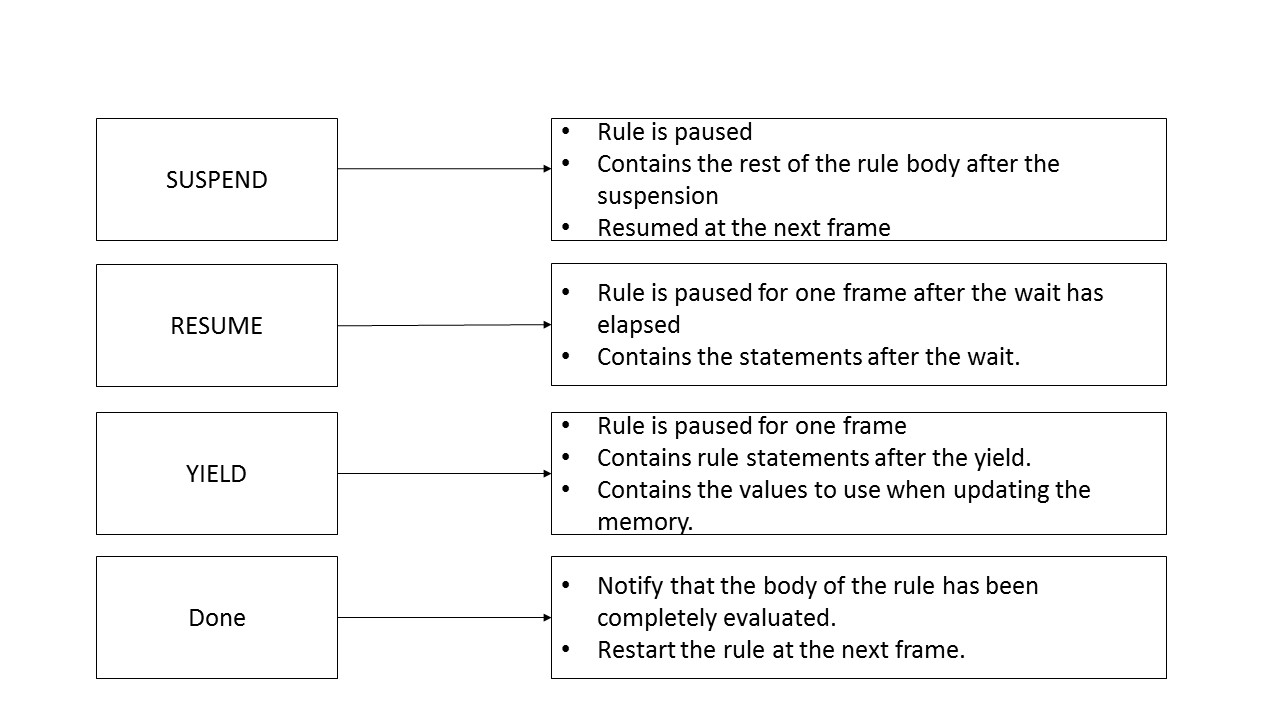
\includegraphics[scale = 0.25]{Pictures/tick2}
	\caption{Casanova 2.5 rule evaluation}
	\label{fig:tick}
\end{figure}

The function \texttt{evalRule} calls \texttt{evalStatement} to evaluate the first statement in the body of the rule passed as argument. The result of the evaluation of the statement is processed in the following way: (\textit{i}) if the result is \texttt{Done}, \texttt{Suspend} or \texttt{Resume} then it is just returned to the caller function. We omit the code for this case, since it is trivial; (\textit{ii}) if the result is \texttt{Atomic} it means that the evaluated statement was uninterruptible and the remaining statements of the rule must be re-evaluated immediately; (\textit{iii}) if the result is \texttt{Yield} then the fields in the domain are updated recursively in order and then the updated memory is encapsulated in the \texttt{Yield} data structure and passed to the caller function.

\vspace{0.1cm}
\begin{lstlisting}
evalStatement b k ctxt dt => Atomic z c    
evalRule (rule dom z nop c dt) => res
-------------------------------
evalRule (rule dom b k ctxt dt)  => res
\end{lstlisting}

\begin{lstlisting}
evalStatement b k (Context locals fields globals) dt => Yield ks values context
updateFields dom values context  => updatedContext
--------------------------------------------------------
evalRule (rule dom b k locals dt) fields globals => Yield ks values updatedContex
\end{lstlisting}

Note that, in case of a rule containing only atomic statements, we will eventually return \texttt{Done} after having recursively called \texttt{evalStatement} for all the statements, and the rule will be paused for one frame.

\begin{comment}
\begin{figure}
	\centering
	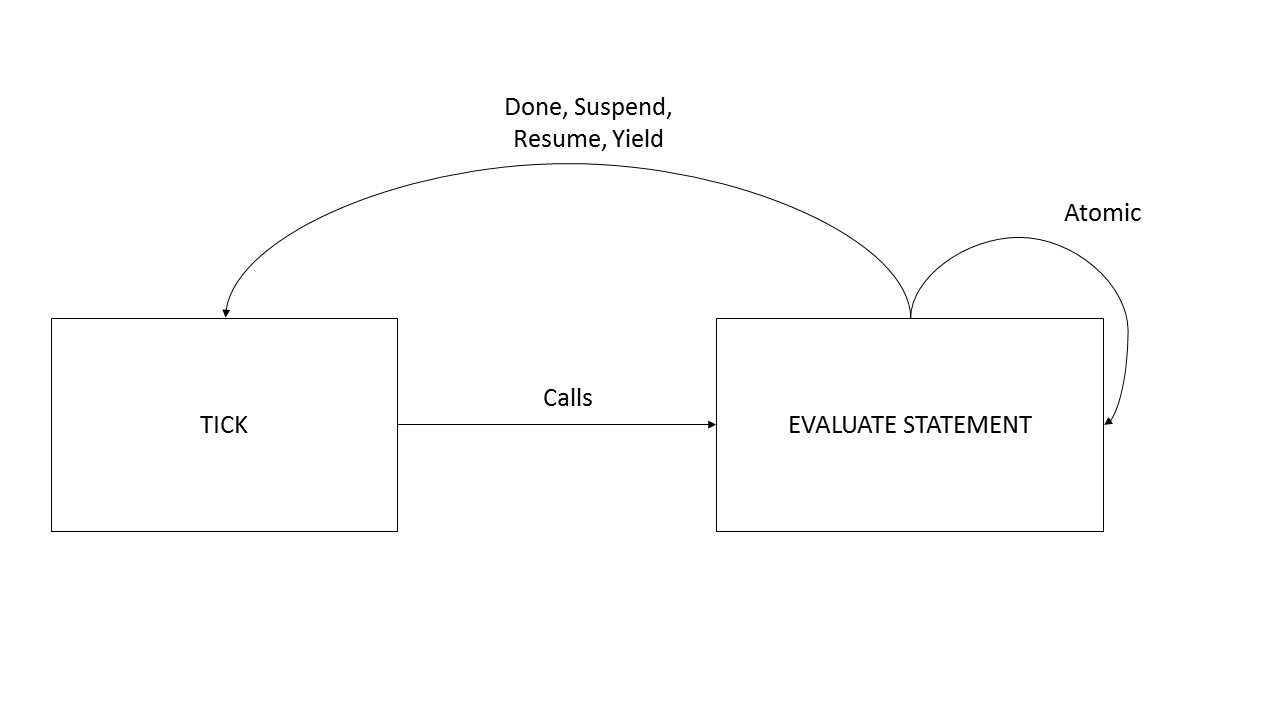
\includegraphics[scale=0.15]{Pictures/statement_evaluation}
	\caption{Statement evaluation}
	\label{fig:statement_evaluation}
\end{figure}
\end{comment}

\noindent
The \texttt{evalStatement} function is used both to evaluate a single statement and a sequence of statements. When evaluating a sequence of statements, the first one is extracted. A continuation is built with the following statement and passed to a recursive call to \texttt{evalStatement} which evaluates the extracted statement. If the existing continuation is non-empty, then it is added before the current continuation. If both the continuation and the body are empty (situation represented by the \texttt{nop} operator) then it means the rule evaluation has been completed and we return \texttt{Done}.

\begin{lstlisting}
a != nop
---------------------                           ----------------------- 
addStmt a b => a;b                              addStmt nop nop => nop   

addStmt b k => cont
evalStatement a cont ctxt dt => res
-------------------------------                 -----------------------------------       
evalStatement (a;b) k ctxt dt => res            evalStatement nop nop ctxt dt => Done ctxt


\end{lstlisting}

\noindent
We will now present, for brevity, only the evaluation of the \texttt{wait} and \texttt{yield} statements. Both the evaluation of the control structures and the variable bindings always return \texttt{Atomic} because they do not, by definition, pause the execution of the rule.

The \texttt{wait} statement has two different evaluations, based on the rules defined in Section \ref{sec:problem_statement}: (\textit{i}) the timer has elapsed: in this case we return \texttt{Resume} which contains the code to execute after the \texttt{wait} statement, or (\textit{ii}) the timer has not elapsed: in this case we return \texttt{Suspend} which contains the \texttt{wait} statement with the updated timer followed by the continuation.


\begin{lstlisting}
<<t <= dt>> == false
----------------------------------
evalStatement (wait t) k ctxt dt => Suspend wait <<t - dt>>;k ctxt

<<t <= dt>> == true
----------------------------------
evalStatement (wait t) k ctxt dt => Resume k ctxt
\end{lstlisting}

\noindent
The \texttt{yield} statement takes as argument a list of expressions whose values are used to update the corresponding fields in the rule domain. The evaluation rule recursively evaluates the expressions and stores them into a list passed as argument of the \texttt{Yield} result. Those arguments are used later by \texttt{evalRule} to update the corresponding fields.

\begin{lstlisting}
eval expr ctxt => v
evalYield exprs ctxt => vs
-------------------------------------------          ----------------------------
evalYield (expr :: exprs) ctxt => v :: vs            evalYield nil ctxt => nil
\end{lstlisting}